\chapter{Network Security}

\section{Background}
\subsection{Protocol}
A protocol is an agreement on a well-defined set of rules for how to communicate or exchange data. It defines the syntax and semantics of communication, e.g., 

- In what format the message shall be structured.  

- In which order the messages shall be sent.  

- What actions need to be taken when receiving or missing a message.  

A network protocol is a set of protocols used to transport data between nodes of a network. For example:

- TCP/IP Protocol Suite  

- Link protocols  

- Internet protocols  

- Transport protocols  

- Application protocols  

\subsection{Networking Stack}
The networking stack can be viewed as layers of protocols, since it is built on top of several protocols at different layers. Layering allows modularization, which simplifies the design of protocols for different tasks. 

Here, different layers just agree on the interface to exchange messages, while the implementation of each layer is independent of that of other layers. A change in the implementation of a layer's service is transparent to the rest of the system. 

Consider TCP/IP layering (Figure 7.1). 

At the physical layer, raw bits are sent over a medium such as cables, Wi-Fi, or fiber. This is just raw transmission without understanding of the message.

Next is the link layer, where data is transferred between neighboring network nodes. This includes protocols like Ethernet and PPP (Point-to-Point Protocol).

Layer 3 is the network layer, which routes packets (datagrams) from source to destination across multiple networks, for example IP (Internet Protocol).

Layer 4 is the transport layer, which ensures end-to-end communication between processes or applications. This uses protocols like TCP and UDP. 

The last one is the application layer, which provides services for applications to use the network, including protocols like HTTP, FTP, and SMTP.

\begin{figure}[H]
  \centering
  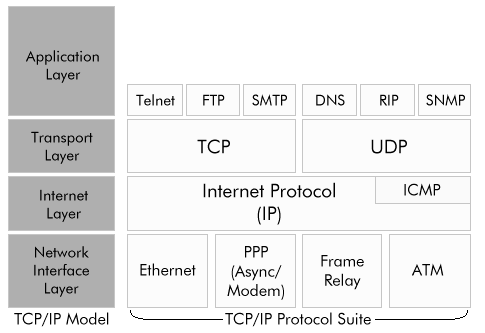
\includegraphics[width=0.5\textwidth]{Figure/TCPIP.png}
  \caption{TCP/IP Layering}
\end{figure}

\subsection{Internet Protocol}
The Internet Protocol is used to provide interconnection of different networks. It provides a connectionless, unreliable, best-effort datagram delivery service, where delivery, integrity, ordering, non-duplication, and bandwidth are all not guaranteed. It relies on a number of different lower-level layer protocols. 

IP datagrams can be exchanged between any two nodes on the Internet. Each network interface has one unique IP address that is globally addressable. IPv4 addresses are composed of 4-byte values, represented in dotted-decimal notation, e.g., \texttt{127.0.0.1}. 

The structure of an IP datagram header is like this:

\begin{figure}[H]
  \centering
  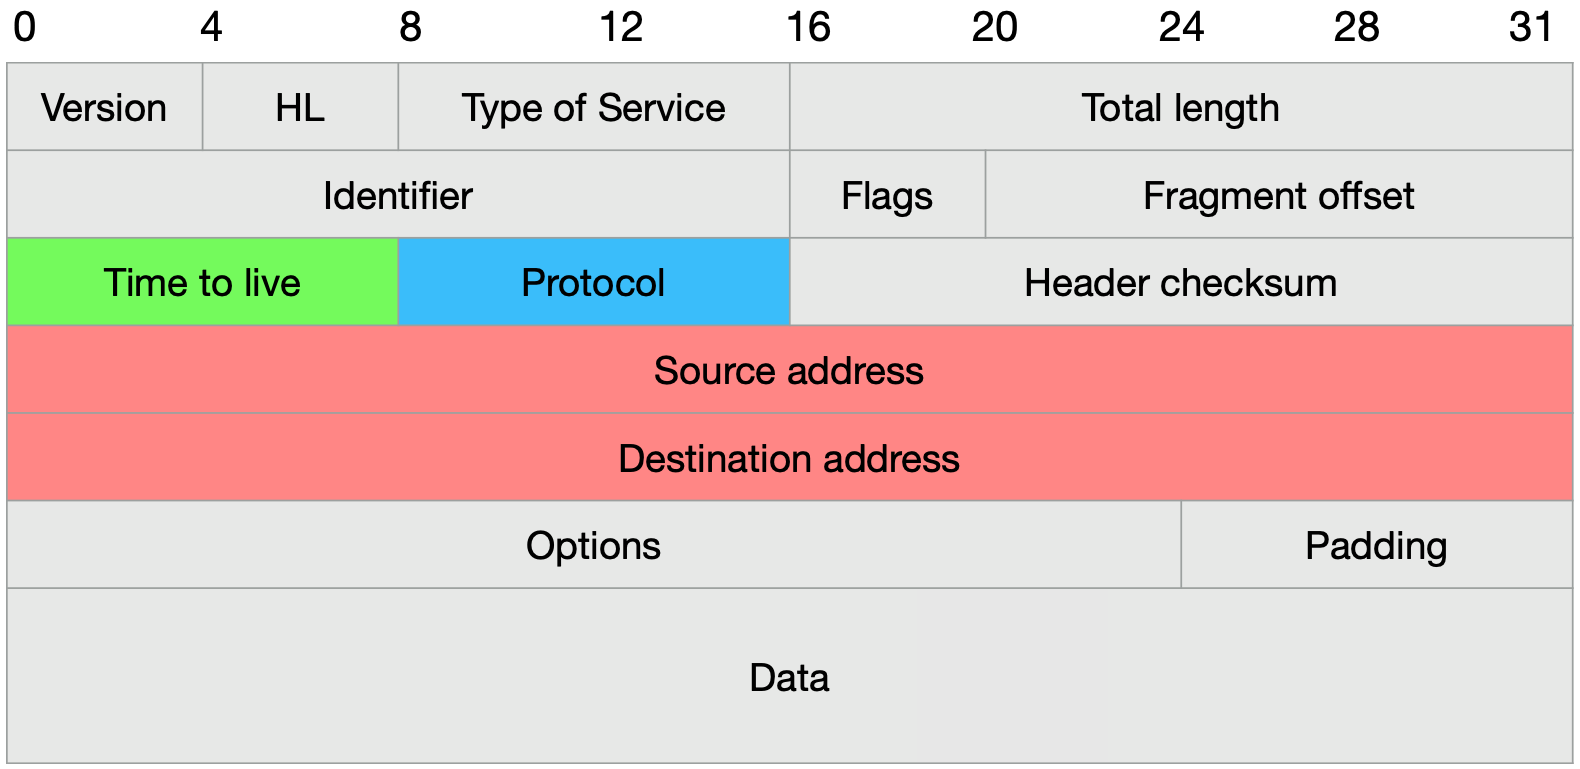
\includegraphics[width=0.7\textwidth]{Figure/IPDatagram.png}
  \caption{IP Datagram}
\end{figure}

where we have

\textbf{Basic Information}

- Version: IP version (IPv4 = 4)  

- HL: Header Length  

- Total Length: Size of entire datagram (header + data)  

\textbf{Handling \& Priority}

- Type of Service: Priority / quality (e.g., delay-sensitive traffic)  

\textbf{Fragmentation}

- Identifier: ID to group fragments of the same packet  

- Flags: Control fragmentation (e.g., “more fragments coming”)  

- Fragment Offset: Position of this fragment in the original data  

\textbf{Lifetime Control}

- Time To Live: Maximum number of hops (routers), decreases at each hop  

\textbf{Upper-layer Information}

- Protocol: Indicates what is inside the data  

\textbf{Error Checking}

- Header Checksum: Detects errors in the header  

\textbf{Addressing} 

- Source Address, Destination Address  

\textbf{Optional}

- Options, Padding  

If two hosts are in the same physical network, the IP datagram is delivered directly within the network (intra-network communication) using a switch, by encapsulating it in a lower-level protocol, for example, as an Ethernet packet (Figure 7.3).

If two hosts are in separate physical networks, the IP datagram is forwarded through intermediate devices, with routers handling inter-network communication between networks.

Ethernet is a link-layer protocol that is widely used in LANs\footnote{Local Area Network (LAN) is a network that connects devices in a limited, local area, like a home, office, or school.}. It includes a 2-byte type field, indicating the protocol the frame is carrying, such as IP, ARP, and RARP. It can carry data with a minimum of 46 bytes and a maximum of 1500 bytes. It also includes a Cyclic Redundancy Check that checks for errors, which occupies 4 bytes. 

\begin{figure}[H]
  \centering
  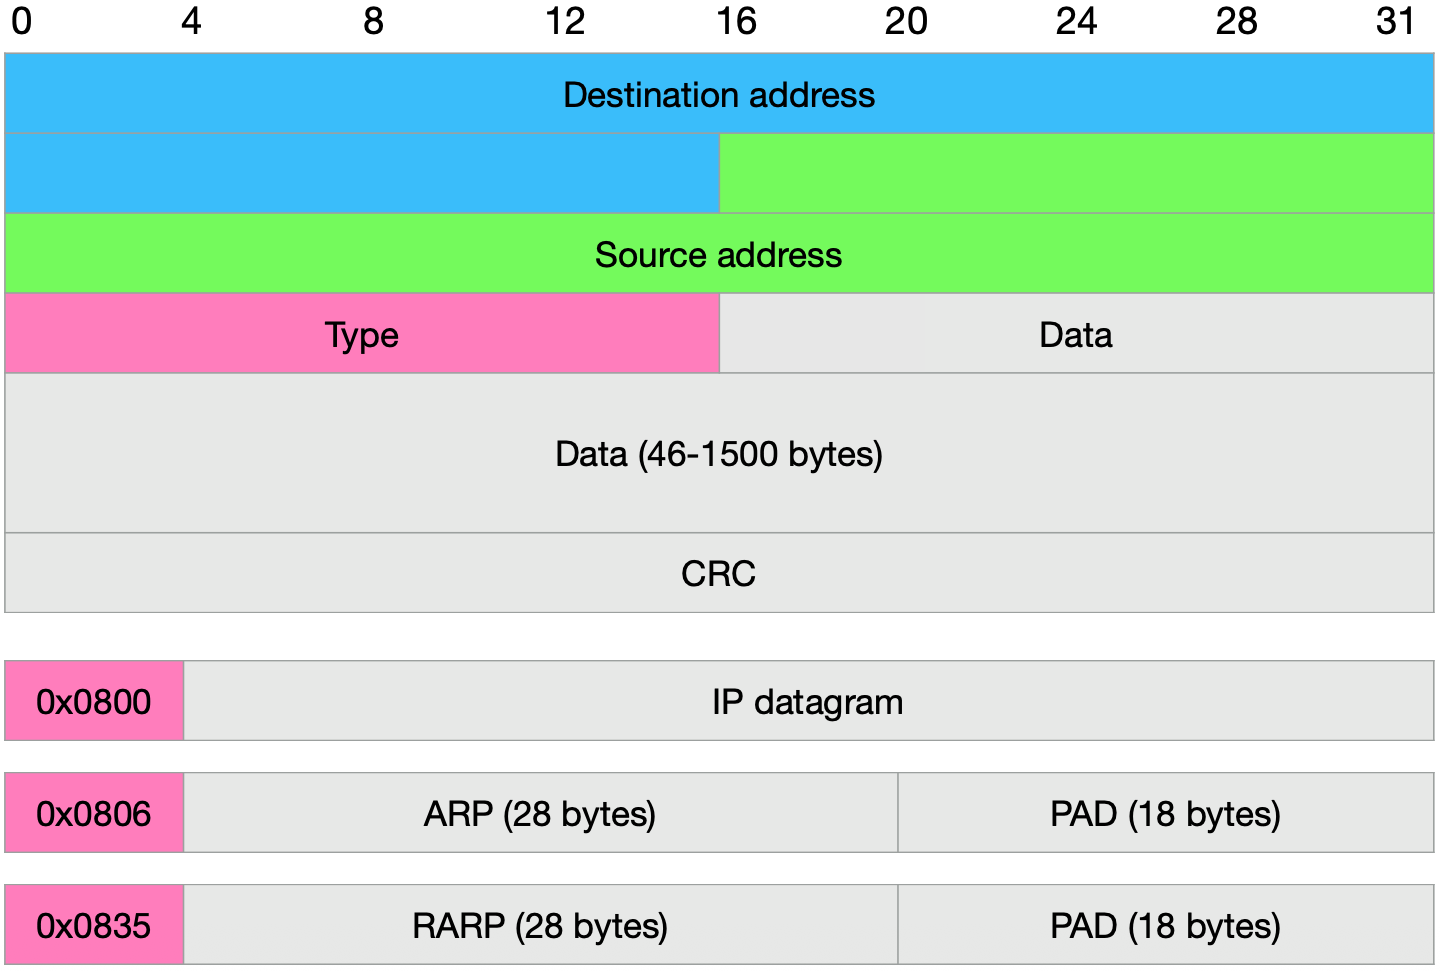
\includegraphics[width=0.7\textwidth]{Figure/EthernetFrame.png}
  \caption{Ethernet Frame}
\end{figure}

Switches are widely used to connect machines in a LAN. It is a device that stores and forwards Ethernet frames, examines incoming frames' MAC addresses, and selectively forwards frames to one or more outgoing links. It also has a self-learning mapping of ports and MAC addresses, i.e., it builds and maintains a table with MAC address-to-port mappings. It learns the mapping from incoming frames, so no manual configuration is needed (plug and play). Multiple packets can be switched simultaneously. 

\section{Local Area Network Attacks}
The goals of these attacks include the following:

- Impersonation of a host

- Denial of service

- Access to information

- Tampering with delivery mechanisms

\subsection{Network Sniffing}
Sniffing (or eavesdropping) refers to the activity of gathering traffic from the local network. This technique forms the basis of many attacks. 

Sniffing can be done by putting a network interface in promiscuous mode to listen to all transmissions, even if the destination address is not that of the attacker. Attackers can then see all data from the link layer up to the application layer. If switched Ethernet is used, the switch must be ``convinced'' to send a copy of the traffic to the port of the sniffing host. 

As many protocols (FTP, POP, HTTP, IMAP) transfer data, including authentication information, in the clear (without encryption), sniffing can allow attackers to collect credentials, emails, files, and more. Sniffing is also used by administrators to monitor network behavior. 

There are sniffing tools that collect, analyze, and replay traffic. These are routinely used for traffic analysis and troubleshooting. For example, command-line tools include:

- \texttt{tcpdump}: collects traffic

- \texttt{tcpflow}: reassembles TCP flows for analysis

- \texttt{tcpreplay}: re-sends recorded traffic

GUI tools include Wireshark. 

Sniffers are typically passive programs. They can be detected by programs that provide information on the status of a network interface. However, a kernel-level rootkit can easily hide the presence of a sniffer.

\subsection{Spoofing}

\subsubsection{Address Resolution Protocol (ARP)}
A host usually has two types of addresses:

- \textbf{Hardware address:} link-layer address 

- \textbf{IP address:} network-layer address  

Host A can determine the MAC address of host B using the Address Resolution Protocol (ARP). ARP allows a host to map an IP address to the link-layer address associated with the peer's hardware interface, enabling direct delivery of packets. 

Each node maintains an ARP table that stores IP-to-hardware address mappings. If host A wants to know the hardware address associated with host B's IP, it can either:

- Check the hardware address in its ARP table  

- Broadcast a message to all hosts on the same local network; host B will respond with its link-level address  

ARP messages are encapsulated in the underlying link-layer protocol.  

\subsubsection{ARP Spoofing}
The goal of ARP spoofing is to sniff all traffic between two hosts in a switched environment. The attack exploits the stateless nature of ARP, where replies without a corresponding request are accepted. 

For example, an attacker sends spoofed ARP messages (request or reply) to the two victim hosts, poisoning their ARP caches. The victim hosts then send their IP packets to the attacker, who can act as a router, intercepting and potentially modifying traffic.  

\subsubsection{Defense}
To defend against ARP spoofing, the following methods can be used:

1. \textbf{Static ARP entries:}  

Configure the ARP cache to ignore dynamic updates. This is difficult to manage in large deployments.  

2. \textbf{Cache poisoning resistance:}  

Ignore unsolicited ARP replies. Updates on timeout can also limit poisoning, but this approach has limited usefulness.  

3. \textbf{Monitor changes (e.g., arpwatch):}  

Tools like arpwatch listen for ARP packets on a local Ethernet interface, track Ethernet/IP address pairs, and report suspicious activity or changes in mapping.  

\subsection{Hijacking}
Sniffing and spoofing form the basis for hijacking attacks. The attacker monitors the network for a client request and races legitimate hosts to send a malicious reply. Hijacking can be based on ARP, UDP, or TCP.  

\subsubsection{Dynamic Host Configuration Protocol (DHCP)}
A new host initially has no IP address (source IP) and does not know which server to contact (no destination IP). DHCP dynamically allocates IP addresses to hosts. The host broadcasts a server-discovery message on the link layer to find available servers, and a DHCP server responds with an address offer.  

The DHCP server also provides:

- DNS server information  

- Gateway address (first hop for all Internet traffic)  

- Lease duration  

Local attackers can intercept the broadcast message and send a forged reply, racing the legitimate DHCP server. The attacker can potentially control the DNS server and gateway used by the victim.  

Since the gateway is the first hop for all Internet traffic, an attacker controlling it can sniff, intercept, block, or modify traffic.  

\subsubsection{DHCP Hijacking}
Threats include:

- \textbf{Fake DNS server:} redirects DNS lookups to an attacker-controlled host  

- \textbf{Fake gateway router:} intercepts all Internet traffic of a victim, allowing relay and modification of content between host and remote machines  

Defense is difficult due to the lack of a trust anchor. Broadcast protocols are inherently at risk from local attackers who can sniff, spoof, and hijack communication. Clients are particularly vulnerable during initialization, before any trust relationships are established.  

To secure a LAN, typical assumptions include keeping attackers out of the LAN. Additional defenses include smart switching and active monitoring:

- Avoid broadcasting all traffic (unlike hubs)  

- Forward Ethernet frames only to the corresponding port  

- Filter requests to specific ports to limit which systems can listen  

- Filter replies to limit which systems can respond  